%!TEX root = main.tex


Fingerprints are ridge and valley patterns presented on the surface of human fingertips.
%
Fingerprints are used to recognize humans for applications such as verifying an identity claim (\textit{i.e.}, one-to-one search to  unlock a smartphone, for example), or identification (\textit{i.e.}, one-to-many search to find a suspect of a crime, for instance).
%
Typically, to query a fingerprint, a system needs to search and compare the query print with the fingerprints stored in its reference (or enrolled) database.  The size of a reference database can be from thousands to hundreds of millions of subjects, depending on the application. For example, the Aaddhar project in India has enrolled 111,98,29,743 persons as of February 18, 2017 \cite{aaddhaar}.  
%
As the size of the database grows, the number of comparisons to be made for identification purposes grow, so does the computation time.
%
To mitigate this problem, most fingerprint recognition algorithms first classify a fingerprint into a basic pattern type and then perform fingerprint matching within fingerprints of that type.
%
The major five fingerprint pattern types used today are an extension of the three pattern types (whorl, loop, and arch) introduced by Henry Faulds (Henry classification system \cite{henry1905classification}) and Sir Francis Galton \cite{galton1892} in late 19th century. These five pattern types are: arch, left loop, right loop, tented arch and whorl, see Figure\ref{fig.fingerprint_classes}.  
%
The Fingerprint Source Book \cite{nijSourceBook} defines each of these patterns as follows: 
%
Arch is a pattern type in which the friction ridges enter on one side of the impression and flow, or tend to flow, out the other side with a rise or wave in the center. 
%
Tented arch is a pattern type that possesses either an angle, an upthrust, or two of the three basic characteristics of the loop. 
%
Loop is a pattern type in which one or more friction ridges enter upon one side, recurve, touch or pass an imaginary line between delta and core and flow out, or tend to flow out, on the same side the friction ridges entered. Loops can be left slant loops (or left loops), in which the pattern flows to the left in the impression; or right slant loops (right loops), in which the pattern flows to the right in the impression.
%
Whorl is a fingerprint pattern type that consists of one or more friction ridges that make, or tends to make, a complete circuit, with two deltas, between which, when an imaginary line is drawn, at least one recurving friction ridge within the inner pattern area is cut or touched. 

As mentioned above, to manage the computation load, large scale fingerprint identification algorithms employ multi-stage matching whose first step is often filtering based on fingerprint pattern type.\footnote{Some of more recent fingerprint classification algorithms use continuous classifications instead of discrete classes. These continuous spectrums are beyond the scope of this paper because of their non-intuitive and proprietary nature as they are developed for a dedicated recognition algorithm.} As such the accuracy of the fingerprint classification algorithm largely influences the identification accuracy. An error in finger pattern classification will propagate throughout the system, and ultimately result in an recognition error. 
Challenges in fingerprint pattern classification include: 
%
1) quality of fingerprints, characterizing poor quality images are particularly difficult,
%
2) small inter-class dissimilarity and small intra-class similarity, for example, tented arch and loop may look similar; 
%
3) ambiguities in some pattern class labels, some fingerprints can be classified into multiple classes, or different classes by different fingerprint experts.

In this paper we propose an automated fingerprint pattern classification that unlike previous finger pattern classifiers, does not require feature extraction.  Specifically, we trained a deep convolutional neural network to take a fingerprint image as an input and classify it into one of the five pattern class types of a) Arch; b) Tented Arch; c) Left Loop; d) Right Loop; or e) Whorl. 

The rest of the paper is organized as follows.  Section \ref{sec_motivtn} overviews previous work. 
Section \ref{sec_method} details our technical approach. 
We describe our experimental set up, data and results in Section \ref{sec_exp}.
Finally, we conclude in Section \ref{sec_con} and present our suggested way forward.

\begin{figure}[!ht]
	\begin{center}
		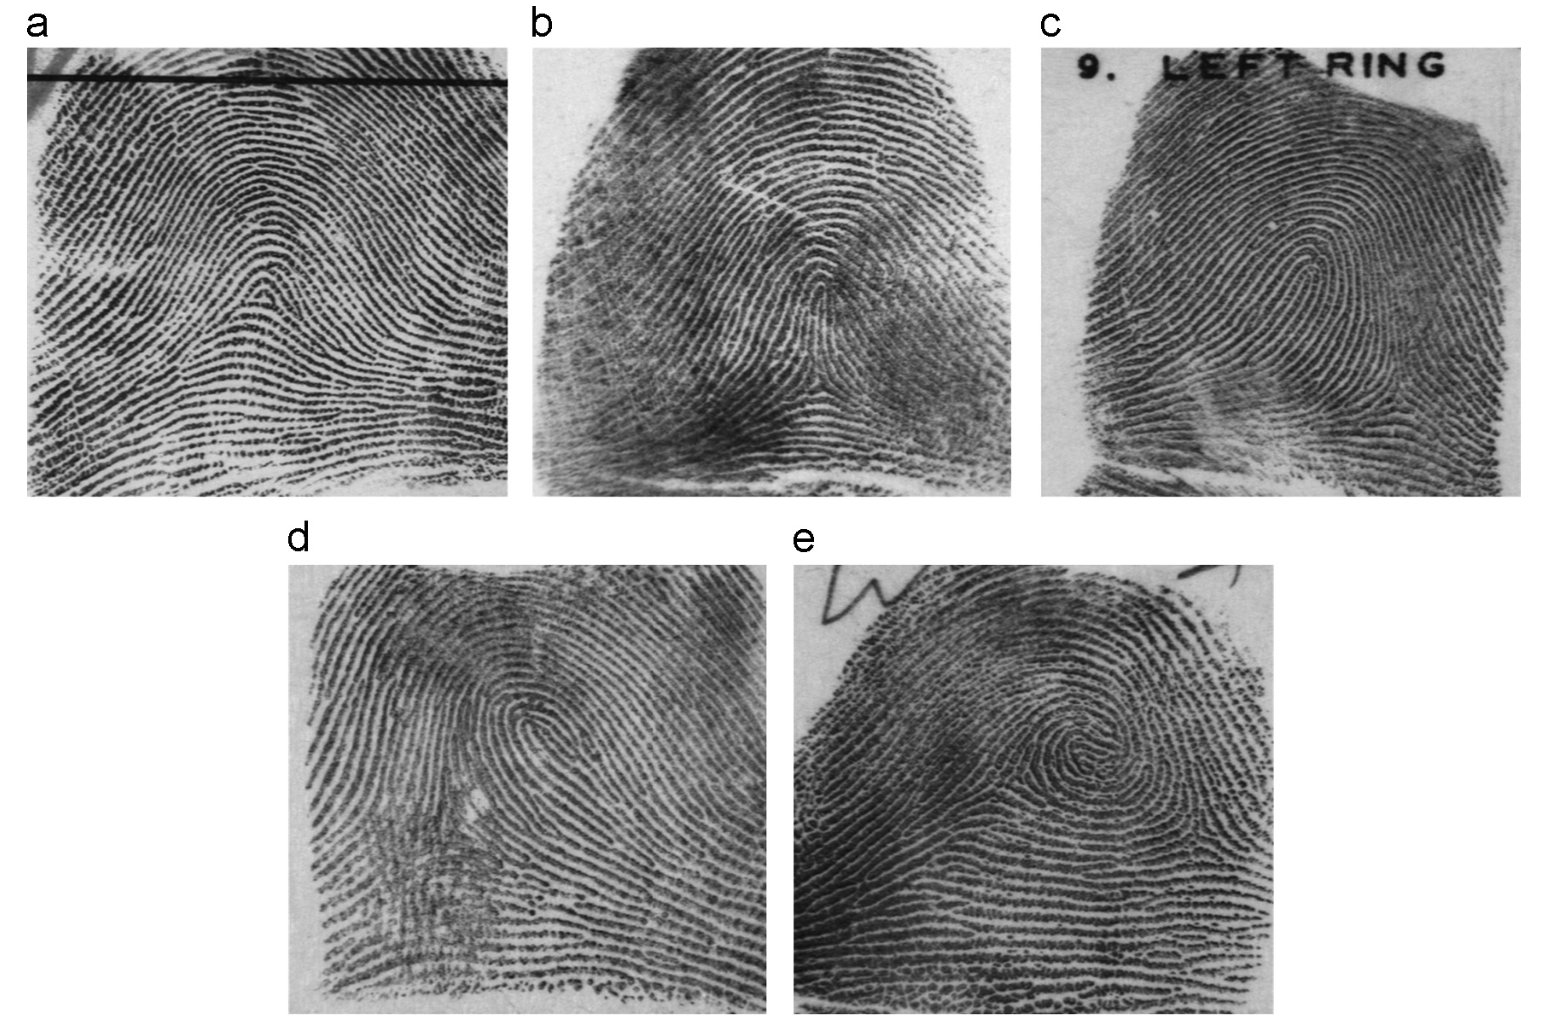
\includegraphics[width=8cm]{fig/Fingerprint_classes.png}
	\end{center}
	\caption{Examples of fingerprint classes\cite{cao2013fingerprint}: (a) Arch, (b) Tented Arch,  (c) Left Loop, and  (d) Right Loop.  Because arch and tented arch only accounts for a small portion in human, most often they are combined into one class.} 
	\label{fig.fingerprint_classes}
\end{figure}

